\documentclass[a4paper, 10pt]{article}
\usepackage[left=2.5cm,top=3cm,right=2.5cm,bottom=2.5cm]{geometry}


\usepackage[utf8]{inputenc}
\usepackage{ragged2e}  
\usepackage{cancel}
\usepackage{mathrsfs}
\usepackage{amsmath}
\usepackage{graphicx}
\usepackage{array}
\usepackage{hyperref}
% \usepackage[spanish]{babel}
\usepackage{multicol}
\usepackage{amssymb}
\usepackage[usenames,dvipsnames,svgnames,table]{xcolor}
\usepackage{dsfont}
\usepackage{parskip}

\begin{document}
	
	La mínima escala de la cinta métrica es $\dfrac{0.1 cm}{2}=0.05 cm$
	
	Los resultados obtenidos al realizar el experimento fueron los siguientes (ver tabla 1)
	
	\begin{table}[ht]
		\centering
		\caption{Resultados obtenidos de las mediciones.}
		\begin{tabular}{|c|c|}
			\hline
			Posición de la lente objetivo & $ (43.15\pm0.05)cm $ \\
			\hline
			Posición de la lente ocular & $ (14.85\pm0.05)cm $  \\
			\hline
			Posición de la pantalla & $ (70\pm0.05) cm $  \\
			\hline
			Magnificación observada & $ 1:2 $ \\
			\hline
			$d_{o1}$ & $ (26.85\pm 0.05) cm $  \\
			\hline
			$d_{i2}$ & $ (-32.3916\pm 0.2871) cm $ \\
			\hline
			$d_{i1} $ & $ (15.9347\pm0.0769)cm $  \\
			\hline
			$d_{o2}$ & $ (12.3652\pm0.1769)cm $  \\
			\hline
			Magnificación calculada & $ -1.5546\pm0.0464 $  \\
			\hline
			Error absoluto &  $ |2-1.5546|=0.4453 $\\
			\hline
		\end{tabular}
	\end{table}
	
	El trazo de rayos con los datos obtenidos queda de la siguiente manera
	
	\begin{figure}[ht]
		\centering
		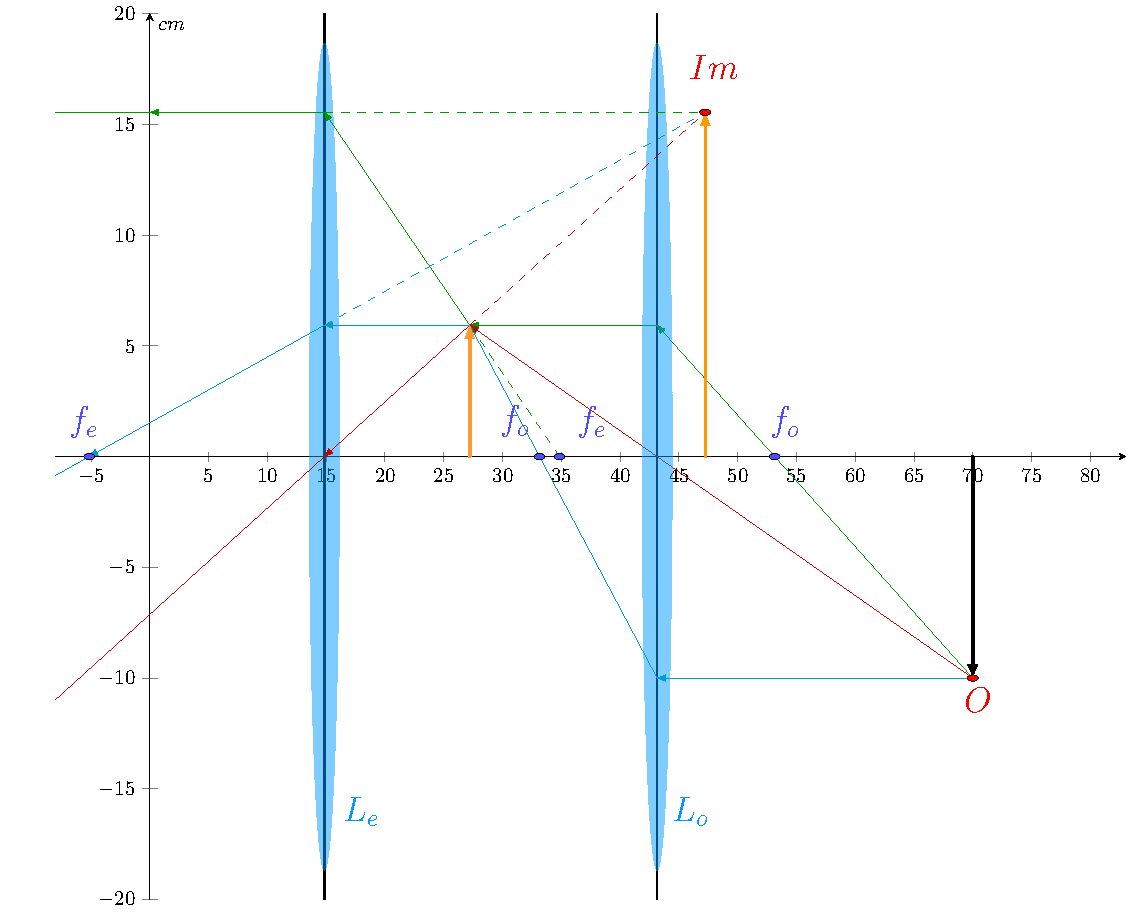
\includegraphics[height=12cm]{rayos.pdf}
		\caption{Trazado de rayos para el microscopio con las condiciones del laboratorio.}
	\end{figure}
	
%	\begin{center}
%		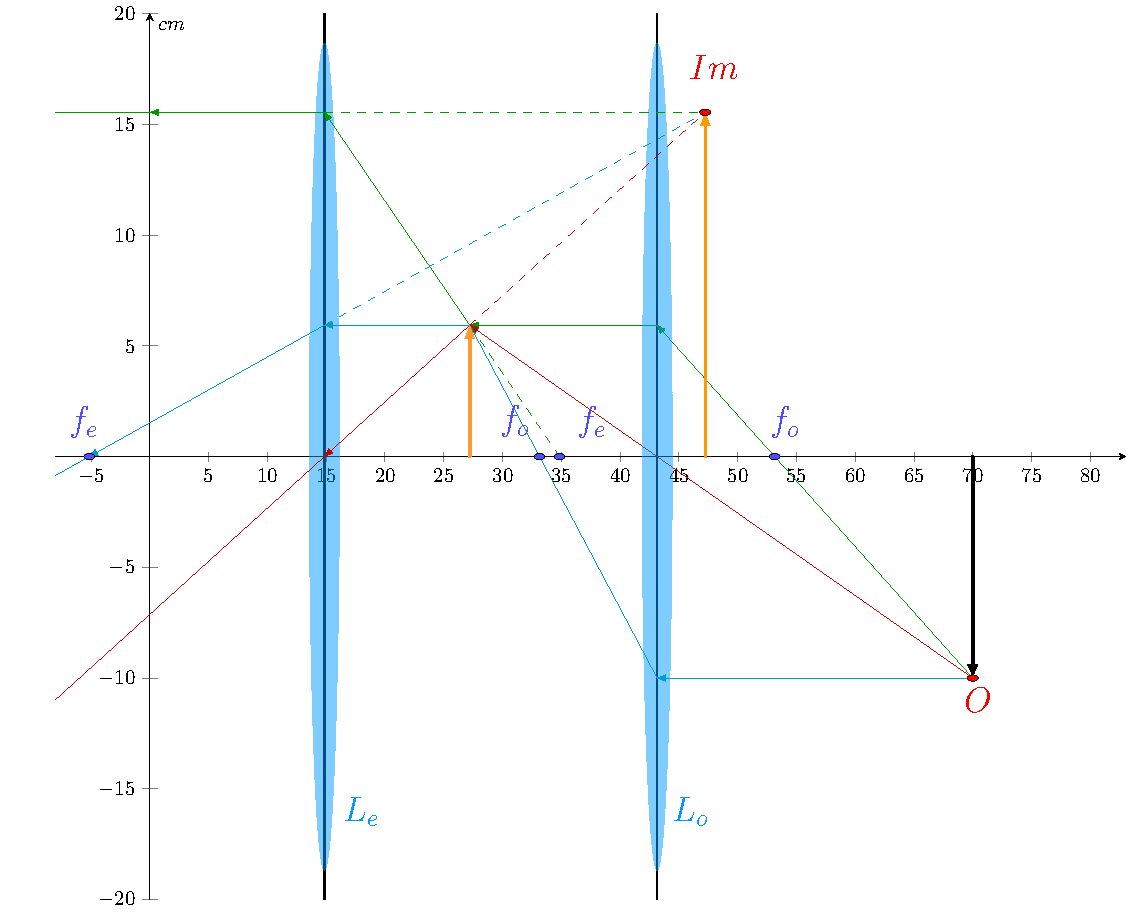
\includegraphics{rayos.pdf}
%	\end{center}
	
	
	
	\newpage
	APÉNDICE
	
	De la fórmula de lentes delgadas se sabe que 
	$$\dfrac{1}{d_o}+\dfrac{1}{d_i}=\dfrac{1}{f}$$
	Despejando $ d_i $ se tiene: \hspace{0.4cm} $d_i=\dfrac{d_o\cdot f}{d_o-f}$
	
	Por otro lado, la incertidumbre para la suma, el producto y un cociente están dadas (respectivamente) por
	\begin{align*}
		(x\pm \delta x)\pm(y\pm \delta y)&=(x\pm y)\pm(\delta x+\delta y)\\\\
		(x\pm\delta x)(y\pm\delta y)&=x\cdot y\pm\left(|y|\delta x+|x|\delta y \right)\\\\
		\dfrac{x\pm\delta x}{y\pm\delta y}&=\dfrac{x}{y}\pm\left(\dfrac{\delta x}{|y|}+|x|\dfrac{\delta y}{|y|^2}\right)
	\end{align*}
	
	Haciendo los cálculos para $ d_{i1} $
	
	\begin{align*}
		d_{o1}\cdot f_1&=[(26.85\pm 0.05)cm](10cm)=\\	&=[(26.85\cdot10)\pm(0.05\cdot20)]cm^2=\\
		&=(268.5\pm0.5)cm^2\\\\
		d_{o1}-f_1&=[(26.85\pm 0.05)cm]-(10cm)=\\
		&=(16.85\pm0.05) cm
	\end{align*}
	
	Entonces
	\begin{align*}
		d_{i1}&=\dfrac{d_{o1}\cdot f_1}{d_{o1}-f_1}=\\\\
		&=\dfrac{(268.5\pm0.5)cm^2}{(16.85\pm0.05) cm}=\\\\
		&=\left[\dfrac{268.5}{16.85}\pm\left(\dfrac{0.5}{16.85}+
		268.5\cdot\dfrac{0.05}{16.85^2}\right)\right]cm=\\\\
		&=(15.9347\pm0.0769)cm
	\end{align*}
	
	Ahora, para la distancia objeto con respecto a la lente ocular ($ L_e $), se tiene que
	
	\begin{align*}
		d_{o2}&=(d_{L_o}-d_{i1})-d_{L_e}=\\
		&=[(43.15\pm0.05)cm-(15.9347\pm0.0769)cm]-(14.85\pm0.05)cm=\\
		&=(27.2152\pm0.1269)cm-(14.85\pm0.05)cm=\\
		&=(12.3652\pm0.1769)cm
	\end{align*} 

	
	Entonces, ahora haciendo los cálculos para obtener $d_{i2}$
	\begin{align*}
		d_{o2}\cdot f_2&=[(12.3652\pm0.1769)cm](20cm)=\\
		&=\left[(12.3652\cdot20)\pm\left(0.1769\cdot20\right)\right]cm^2=\\
		&=(247.304\pm3.538)cm^2\\\\
		d_{o2}-f_2&=(12.3652\pm0.1769)cm-(20cm)=\\
		&=(-7.6348\pm0.1769)cm
	\end{align*}

	Así pues 
	\begin{align*}
		d_{i2}&=\dfrac{d_o2\cdot f_2}{d_o2-f_2}=\dfrac{(247.304\pm3.538)cm^2}{(-7.6348\pm0.1769)cm}=\\\\
		&=\left[\dfrac{247.304}{-7.6348}\pm\left(\dfrac{3.538}{7.6348}+247.304\cdot\dfrac{0.1769}{7.6348^2}\right)\right]cm=\\\\
		&=(-32.3916\pm 0.2871)cm
	\end{align*}

	Los cálculos correspondientes para $M1$ son los siguientes
	\begin{align*}
		M1&=-\dfrac{d_{i1}}{d_{o1}}=-\dfrac{(15.9347\pm0.0769)cm}{(26.85\pm 0.05) cm}=\\\\
		&=-\dfrac{15.9347}{26.85}\pm\left(\dfrac{0.0769}{26.85}+15.9347\cdot\dfrac{0.05}{26.85^2}\right)=\\\\
		&=-0.5934\pm0.0039 
	\end{align*}
	Y para $M2$
	\begin{align*}
		M2&=-\dfrac{d_{i2}}{d_{o2}}=-\dfrac{(-32.3916\pm 0.2871) cm}{(12.3652\pm0.1769)cm}=\\\\
		&=-\dfrac{(-32.3916)}{12.3652}\pm\left(\dfrac{0.2871}{12.3652}+32.3916\cdot\dfrac{0.1769}{12.3652^2}\right)=\\\\
		&=2.6195\pm0.0606
	\end{align*}
	
	Con esto, se puede calcular la magnificación total
	\begin{align*}
		M_T=M_1\cdot M_2&=(-0.5934\pm0.0039)(2.6195\pm0.0606)=\\\\
		&=(-0.5934)(2.6195)\pm\left(0.5934\cdot0.0606+2.6195\cdot0.0039\right)=\\\\
		&=-1.5546\pm0.0464 
	\end{align*}
	
\end{document}
